%\documentclass[options]{class}
\documentclass[12pt, twoside]{report}

%Para listado de programas
\usepackage{listings}
\usepackage{color}

\definecolor{mygreen}{rgb}{0,0.5,0}
\definecolor{mygray}{rgb}{0.7,0.7,0.7}
\definecolor{mymauve}{rgb}{0.58,0,0.82}

\lstset{ %
	 backgroundcolor=\color{mygray},   % choose the background color; you must add \usepackage{color} or \usepackage{xcolor}
	 basicstyle=\footnotesize\ttfamily,        % the size of the fonts that are used for the code
	 breaklines=true,            % Zeilen werden Umgebrochen
	 keywordstyle=\color{red},
	 commentstyle=\itshape\color{mygreen},    % comment style
	 numbers=left,                    % where to put the line-numbers; possible values are (none, left, right)
	 numbersep=5pt                   % how far the line-numbers are from the code
}

%Paquete de Idioma
\usepackage[spanish]{babel}

%Codificación Alfabeto
\usepackage[utf8]{inputenc}

%Codificación de Fuente
\usepackage[T1]{fontenc}

%Índice
\usepackage{makeidx}

%Gráficos
\usepackage{graphicx}
\usepackage{float} 
%\usepackage{xcolor} 

%Matemática
\usepackage{amsmath}
\usepackage{amsfonts}
\usepackage{amssymb}
\usepackage{amstext} 

%Estilo de Página Numeración superior
%\pagestyle{headings}

%un estilo propio
\usepackage{fancyhdr}
\setlength{\headheight}{15pt}

\pagestyle{fancy}
\renewcommand{\chaptermark}[1]{ \markboth{\chaptername\ \thechapter: #1}{} }
\renewcommand{\sectionmark}[1]{ \markright{ Sección \thesection. #1}{} }

\fancyhf{}
\fancyhead[LE,RO]{\thepage}
\fancyhead[RE]{\textit{ \nouppercase{\leftmark}} }
\fancyhead[LO]{\textit{ \nouppercase{\rightmark}} }
\fancyfoot[CE]{\textit{\textcopyright 2015 Laboratorio de Sistemas Embebidos\\
	                    UPAEP} }
\fancyfoot[CO]{\textit{LSE004-2015 \\
		Elaboró: Dr. Casimiro Gómez González} }	            
\fancypagestyle{plain}{ %
	\fancyhf{} % remove everything
	\renewcommand{\headrulewidth}{0pt} % remove lines as well
	\renewcommand{\footrulewidth}{0pt}
}

%Hiperlinks \href{url}{text}
\usepackage[pdftex]{hyperref}

\usepackage{cite} % para contraer referencias

%Titulo
\title{LSE004-2015: Programando en el lenguaje RUST}
\author{Dr. Casimiro Gómez González\\
	Facultad de Electrónica, UPAEP\\
               correo: casimiro.gomez@upaep.mx\\
               Tel: 222 229 9428}
\date{Primavera 2015}

\begin{document}

\maketitle

\chapter*{Prólogo}

El presente texto es una introducción a la programación en RUST, incluye las herramientas necesarias para el desarrollo de proyectos de nivel intermedio en este excitante lenguaje y sus aplicaciones en el desarrollo de sistemas embebidos.

\begin{flushright}
	
	El autor\\
	Casimiro Gómez González\\
	Doctor en Ingeniería Mecatrónica \\
	correo: casimiro.gomez@upaep.mx
\end{flushright}

\tableofcontents

\chapter{Instalación de RUST}
Rust es un lenguaje de programación compilado, de propósito general y multiparadigma que está siendo desarrollado por Mozilla. Ha sido diseñado para ser ''un lenguaje seguro, concurrente y práctico'', soportando programación funcional pura, por procedimientos, imperativa y orientada a objetos.

El lenguaje surgió de un proyecto personal desarrollado por Graydon Hoare (trabajador de Mozilla), quién empezó a trabajar en él en 2006; y Mozilla se involucró en este proyecto en 2009 y lo dio a conocer oficialmente en 2010. El mismo año, el trabajo pasó del compilador inicial (escrito en OCaml) al compilador auto contenido, escrito en sí mismo, en Rust. Conocido como rustc, se compiló a sí mismo en 2011. El compilador auto contenido usa LLVM como su back-end.

La primera versión alfa numerada del compilador de Rust apareció en enero de 2012. Según la política de Mozilla, Rust es desarrollado de forma totalmente abierta y solicita la opinión y contribución de la comunidad. El diseño del lenguaje se ha ido perfeccionando a través de las experiencias en el desarrollo del motor de navegador, Servo, y el propio compilador de Rust. Aunque es desarrollado y patrocinado por Mozilla y Samsung, es un proyecto comunitario. Una gran parte de las contribuciones proceden de los miembros de la comunidad.

El objetivo de Rust es ser un buen lenguaje para la creación de grandes programas del lado del cliente y del servidor que se ejecuten en Internet. Esto ha llevado a un conjunto de características con un énfasis en la seguridad, el control de distribución de la memoria y la concurrencia. Se espera que el rendimiento de código seguro sea más lento que C++, si el rendimiento es la única consideración, pero si lo comparamos con el código C++ hecho para que tome precauciones comparables a las que toma Rust, este último puede ser incluso más rápido


\section{Instalando RUST en Linux}

El primer paso para usar Rust es instalarlo. Hay distintas formas de instalar Rust, pero la forma más fácil es usar el script \textbf{rustup}. Se necesita ejecutar el siguiente comando:

\begin{lstlisting}[language=bash]
$ curl -sf -L https://static.rust-lang.org/rustup.sh | sudo sh
\end{lstlisting}

También es posible instalarlo en dos pasos:

\begin{lstlisting}[language=bash]
$ curl -f -L https://static.rust-lang.org/rustup.sh -O
$ sudo sh rustup.sh
\end{lstlisting}


\section{Instalando Rust Nightly}
Se instala Rust Nightly con el siguiente comando:

\begin{lstlisting}[language=bash]
curl -sSf https://static.rust-lang.org/rustup.sh | sudo sh -s -- --channel=nightly --yes
\end{lstlisting}


\subsection{Desinstalando}

Si se desea desinstalar Rust se debe ejecutar el siguiente comando:

\begin{lstlisting}[language=bash]
$ sudo /usr/local/lib/rustlib/uninstall.sh
\end{lstlisting}

\section{Instalación de RustDT}

Para la instalación de RustDT se necesita tener instalado lo siguiente:

\begin{itemize}

 \item Eclipse 4.5 (Mars) or later.
 \item Java VM version 8 or later.
 \item The Racer tool.

\end{itemize}

\subsection{Instrucciones}
\begin{itemize}
\item Usa el Eclipse que tengas instalado en tu sistema o baja el paquete de http://www.eclipse.org/downloads/\footnote{Para un paquete de eclipse sin ningún otro IDE o extra (tal como la herramienta VCS)} debes bajar la "\textit{Platform Runtime Binary}".

\item Iniciar Eclipse, e ir a \textbf{HELP -> Install New Software...}

\item Pulsa el botón \textbf{Add...} para agregar un nuevo sitio, introduce el URL: \textbf{http://rustdt.github.io/releases/} en el campo de localización, pulsa \textbf{OK}.

\item Selecciona el sitio de las actualizaciones recientes en \textbf{work with:} menu. Selecciona \textbf{RustDT} en la caja de opciones. Ahora la característica de \textbf{RustDT} aparecerá en la parte inferior

\item Selecciona la característica \textbf{RustDT} y completa el wizard.\footnote{Las dependencias de \textbf{RustDT} tales como CDT automáticamente  se instalarán durante el proceso de la instalación }

\item Reiniciar Eclipse  

\item Para la configuración inicial sigue las instrucciones en la sección de configuración en la guia de usuario. 

\end{itemize}

\subsection{Actualizar}

Si tienes instalado RustDT y quieres actualizar pulsa \textbf{Help / Check for Updates...}

\chapter{Características Principales de RUST}

RUST es un lenguaje de programación de sistemas enfocado en tres objetivos: Seguridad, velocidad y concurrencia. Se logran estos tres objetivos sin tener un colector de basura, provocando esto que sea un lenguaje útil  para aplicaciones donde otros lenguajes no lo son: Ser embebidos en otros lenguajes, programas con datos específicos de tiempo y espacio, escritura de código de bajo nivel, tales como drivers de dispositivos y sistemas operativos. Mejora de los lenguajes actuales dirigidas a este espacio por tener una serie de controles de seguridad en tiempo de compilación que no producen sobrecarga de tiempo de ejecución , mientras que la eliminación de todas las carreras de datos. Rust también tiene como objetivo lograr `` abstracciones  de costo cero '' a pesar de que algunas de estas abstracciones sienten como los de un lenguaje de alto nivel . Incluso entonces , Rust todavía permite un control preciso como un lenguaje de bajo nivel lo haría.

\section{Una corta introducción a RUST}

EL principal concepto que hace a Rust único es llamado "propiedad". Considere el siguiente ejemplo:

\begin{lstlisting}[language=erlang]
fn main() {
	let mut x = vec!["Hola", "mundo"];
}
\end{lstlisting}

Este programa realiza un enlace de variable llamado \textbf{x}. El valor de este enlace  es un\textit{ Vec<T>}, un ``vector'' a través de una macro definida en la librería estándar. Esta macro es llamada \textbf{vec}, y se invoca a los macros con un \textbf{!}. Esto sigue el principio general de Rust: \textbf{Haz las cosas explícitamente}. Las macros pueden hacer cosas significativamente mas complicadas que las funciones, es por ello que son visualmente distintas. El símbolo \textbf{!} tambien ayuda con el parsing, haciendo la herramienta de macros fácil de escribir, lo cual es muy importante.

Se utiliza \textbf{mut} para hacer \textbf{x} mutable: los enlaces son inmutables por defecto en Rust. 

También vale la pena señalar que no necesitábamos una anotación de tipo aquí: mientras Rust se escribe con tipado estático, no lo necesitamos para anotar explícitamente el tipo . Rust tiene inferencia de tipos para equilibrar el poder de tipos estáticos con el nivel de detalle de la anotación de tipos .

Rust prefiere asignación de pila que asignación de memoria dinámica: x es colocada directamente en la pila. Sin embargo, el tipo Vec<T> coloca espacios para elementos del vector en la memoria dinámica.  Como lenguaje de programación de sistemas, RUST proporciona la habilidad de controlar como las memoria es colocada.

Como mencionamos anteriormente, la ``propiedad'' es el concepto principal en Rust. En el lenguaje Rust, x se dice que es ``Dueño'' del vector. Esto significa que cuando x se elimina, la memoria del vector se descoloca. 
Esto es realizado determinísticamente por el compilador de Rust, mas que a través de un mecanismo tal como el colector de basura. En otras palabras, en RUST, no se llama a la función como \textbf{malloc} y \textbf{free} por ti mismo: El compilador estáticamente determina cuando se necesita colocar o liberar memoria, e introduce estas llamadas por el mismo. Equivocarse es humano, pero el compilador nunca olvida.

Si agregamos otra linea a nuestro ejemplo:

\begin{lstlisting}[language=erlang]
fn main() {
let mut x = vec!["Hello", "world"];

let y = &x[0];
}
\end{lstlisting}

En el programa anterior se introdujo otra ligadura, \textbf{y}. En este caso, \textbf{y} es una ``referencia'' a el primer elemento de el vector. La referencias en Rust son similares a los apuntadores en otros lenguajes, pero con revisiones de seguridad adicionales en tiempo de compilación. Las referencias interactuan con las el sistema de propiedades ``prestando'' a lo que apunta, mas que adueñandose de él. La diferencia es, cuando la referencia se elimina, no será liberada de la memoria. Si así fuera, sería liberada dos veces lo cual es malo.

Ahora adicionemos una tercera línea.

\begin{lstlisting}[language=erlang]
fn main() {
	let mut x = vec!["Hello", "world"];

	let y = &x[0];

	x.push("foo");
}
\end{lstlisting}

\textbf{push} es un método en los vectores que adiciona otro elemento al final del vector. Cuando se trata de compilar este programa, se general el siguiente error:

\begin{lstlisting}[language=erlang]
error: cannot borrow `x` as mutable because it is also borrowed as immutable
x.push(4);
^
note: previous borrow of `x` occurs here; the immutable borrow prevents
subsequent moves or mutable borrows of `x` until the borrow ends
let y = &x[0];
^
note: previous borrow ends here
fn main() {

}
^
\end{lstlisting}

El compilador Rust da información bastante detallada de los errores algunas veces, esta es una de esas veces. Como se señala en el error, mientras hacemos nuestra ligadura mutable no se puede ejecutar  \textbf{push}. Esto es debido a que aún tenemos una referencia a un elemento del vector, \textbf{y}. Mutar algo mientras otra referencia existe es peligroso, porque se podría invalidad la referencia. En este caso específico, cuando creamos un vector, solamente tendremos espacio de memoria para tres elementos. Adicionar un cuarto significa colocar un espacio de memoria para esos elementos nuevos, copiando valores viejos y actualizando el apuntador interno a esa memoria. Todo esto suena bien. El problema es que \textbf{y} no se puede actualizar, por lo que tendremos un apuntador colgante. Esto es malo. Cualquier uso de \textbf{y} generará un error en este caso, así que el compilador captura el error para nosotros.

Asi que ¿Como resolvemos este problema? Se puede utilizando dos técnicas. La primera es haciendo una copia mas que una referencia:


\begin{lstlisting}[language=erlang]
fn main() {
	let mut x = vec!["Hello", "world"];
	
	let y = x[0].clone();
	
	x.push("foo");
}
\end{lstlisting}

Rust tiene una semántica para mover datos, de tal forma que si queremos hacer una copia de alguna dato, llamamos al método \textbf{clone()}. En este ejemplo, \textbf{y} no es más una referencia al vector guardado en \textbf{x\textbf{}}, pero copia su primer elemento ``hola''. Ahora no tenemos referencia, y el método \textbf{push()} trabajará bien.

Si realmente se requiere de utilizar una referencia, se necesita otra opción, esta es: asegurarse que nuestra referencia esta fuera del ambiente antes de que tratemos de hacer la mutación. Esto quería de la siguiente forma:

\begin{lstlisting}[language=erlang]
fn main() {
	let mut x = vec!["Hello", "world"];
	
	{
		let y = &x[0];
	}
	
	x.push("foo");
}
\end{lstlisting}

En este programa se ha creado un ambiente interno utilizando el conjunto de llaves adicionales. \textbf{y} se saca del ambiente antes de llamar al método \textbf{push()}, de tal forma que todo funciona adecuadamente.

El concepto de ``propiedad '' no es bueno para prevenir apuntadores colgados, pero un conjunto de problemas relacionados, como iteracciones inválidas , concurrencia y otros si se previenen.



\section{Programa ``Hola, Mundo''}

Antes de escribir nuestro tradicional programa ``Hola, Mundo'', vamos a crear nuestro subdirectorio de trabajo

\begin{lstlisting}[language=bash]
$ mkdir ~/projects
$ cd ~/projects
$ mkdir hello_world
$ cd hello_world
\end{lstlisting}

Ahora haremos un nuevo archivo fuente. Y llamaremos al archivo \textbf{main.rs}. Los archivos en Rust siempre terminan con la extensión \textbf{.rs}. Si utilizas mas de una palabra en el nombre de tu archivo, se recomienda usar un guión inferior \textbf{Hola\_Mundo.rs} mas que \textbf{HolaMundo.rs}.

Ahora, una vez el archivo este abierto, escribir el siguiente código dentro:

\begin{lstlisting}[language=erlang]
fn main() {
	println!("Hola, Mundo");
}
\end{lstlisting}

Grabar el archivo, y luego escribir los siguientes comandos en la terminal:
\begin{lstlisting}[language=bash]
$ rustc main.rs
$ ./main 
Hello, world!
\end{lstlisting}

¡Éxito! Ahora analizaremos el programa en detalle

\begin{lstlisting}[language=erlang]
fn main() {

}
\end{lstlisting}

Estas lineas definen una función en Rust. La función \textbf{main} es especial: Es el principio de todo programa Rust. La primera linea dice ``Estoy declarando una función llamada \textbf{main} la cual no necesita argumentos y no regresa nada". Si necesitara algún argumento estos irían dentro de los paréntesis, y debido a que no estamos regresando nada se puede omitir la palabra clave \textbf{return} completamente.

\section{Conviertiendo a Cargo}

Vamos a convertir el programa ``Hola Mundo'' a Cargo, para ello necesitamos hacer tres cosas: 

\begin{itemize}
\item Hacer el archivo de configuraciòn \textbf{Cargo.toml}
\item Poner los archivos fuentes en los directorios adecuados
\item Ejecutar el archivo creado
\end{itemize}

\subsection{Primer paso}

\begin{lstlisting}[language=bash]
$ mkdir src
$ mv main.rs src/main.rs 
$ rm main 
\end{lstlisting}

Si deseamos crear una librería en lugar de un ejecutable, debemos usar el nombre lib.rs. Esta convención es usada por Cargo para compilar exitosamente nuestros proyectos. Localizaciones propias pueden ser especificadas con las palabras claves [bin] o [lib] en el archivo TOML.

Cargo espera que tus archivos fuentes se encuentren en el directorio \textbf{src}. Esto deja los archivos de nivel alto para otras cosas, como READMEs, información de licencias, y cualquier otra cosa no relacionado con tu código. Cargo te ayuda a mantener tus proyectos agradables. Un lugar para cada cosa y cada cosa en su lugar.

Ahora, nuestro archivo de configuración:

\chapter{Diseñando el Sistema Operativo \textbf{\textit{UtVitam}} con Rust}

En este trabajo se supondrá que se utilizá un sistema operativo parecido a Unix como plataforma de diseño, como por ejemplo Linux.

\section{Construyecto un \textbf{Cross-Compiler}}
Hay un convención llamada ``el triple objetivo'' para describir una plataforma en particular. Es triple porque consta de tres partes:

\begin{lstlisting}[language=bash]
arch-kernel-userland
\end{lstlisting}
Así que, un triple objetivo para una computadora que tiene un procesador x86-64 bit ejecutando un kernel de linux y programas de usuario (userland) de GNU se vería así:

\begin{lstlisting}[language=bash]
x86_64-linux-gnu
\end{lstlisting}
Si esta compuesto por cuatro partes, se le llama ``Objetivo" mas que ``triple objetivo".

Los kernels por si mismos no necesitan ser para un específico conjunto de programas de usuario, y por eso tu verás 'none' :

\begin{lstlisting}[language=bash]
x86_64-unknown-none
\end{lstlisting}

\subsection{Anfitrión y Objetivos}

La razón por los cuales son llamados ``objetivos'' es porque es la arquitectura para la cual estas compilando. La arquitectura desde la cual compilas se llama ``Arquitectura Anfitrión''.

Si el objetivo y el anfitrión son los mismos, nosotros los llamamos ``Compilación''. Si son diferentes, entonces se llama ``Compilación cruzada''. Así se puede afirmar:


 \begin{flushright}
 \textbf{Compile cruzado desde x86\_64-linux-gnu a x86-unknown-none}
 \end{flushright}

Esto significa que la computadora de desarrollo fue una con GNU/linux de 64 bits, pero el binario final es para una máquina x86 de 32 bits sin sistema operativo.

Por lo tanto se necesita un ambiente en particular construir nuestro Sistema Operativo: Se necesita un compilador cruzado desde cualquier tipo de computadora se este usando para nuestro objetivo.

Para instalar en linux debian o ubuntu, se necesita ejecutar lo siguiente:

\begin{lstlisting}[language=bash]
sudo apt-get install nasm xorriso qemu build-essential
\end{lstlisting}

Lo primero que se debe realizar es configurar un Cross-Compiler para la plataforma \textbf{arm-none-eabi}. No serás capaz de compilar correctamente tu sistema operativo sin un \textit{Cross compiler}. Ahora necesitamos compilar \textbf{libcore} de Rust a nuestra arquitectura objetivo . Se trata de una base mínima libre de la dependencia de la biblioteca estándar. Para eso es necesario para compilar desde el código fuente :

\begin{lstlisting}[language=bash]
git clone https://github.com/rust-lang/rust.git
cd rust
rustc --version   #Se toma el numero que este comando y se introduce despues del comando checkout de la linea siguiente
git checkout 21922e1f4
sudo mkdir -p /usr/local/lib/rustlib/arm-unknown-linux-gnueabihf/lib 
sudo rustc --target arm-unknown-linux-gnueabihf -O -Z no-landing-pads src/libcore/lib.rs --out-dir /usr/local/lib/rustlib/arm-unknown-linux-gnueabihf/lib
\end{lstlisting}

\subsection{Raspberry Pi bootloader}

En el caso de las Raspberry Pi, dos archivos pueden ser encontrados en https://github.com/raspberrypi/firmware/tree/master/boot, el \textbf{bootcode.bin} y el \textbf{start.elf}
Teniendo un SDCARD de arranque se le borran todos los archivos y se colocan los dos:  \textbf{bootcode.bin} y \textbf{start.elf} en la partición \textbf{boot} de la tarjeta

\subsection{Comenzando la programación}

Con todo configurado, podemos empezar a escribir el código. Vamos a hacer que el led ACT de la Raspberry parpadee, es el verde que se encuentra a lado del led de encendido. Así que, nuestro programa, básicamente necesita encender el led, esperar un tiempo, y apagarlo y luego ciclarse. Asi que en un editor creamos el archivo \emph{kernel.rs}:

\begin{lstlisting}[language=erlang]
fn main() {
	println!("Hola Mundo!");
}
\end{lstlisting}

Este es el ejemplo estandar de hola mundo, pero la macro \textbf{println!} es parte de la librería estandar de Rust y usa la plataforma E/S para imprimir algo en la pantalla y en este momento no tenemos ninguna plataforma definida. De tal manera, que necesitamos informarle al compilador que nuestro código independiente será independiente:

\begin{lstlisting}[language=erlang]
#![feature(no_std)]
#![crate_type = "staticlib"]
#![no_std]

// kernel.rs
fn main() {  
    println!("Hola Mundo!");
}
\end{lstlisting}

En la primera linea le informamos al compilador que vamos a usar una característica \textbf{no\_std}, esto se realiza con el atributo  \textbf{\#![feature()]} el cual le informa este tipo de caracteríticas al compilador. Con la instrución \textbf{\#![crate\_type]} le informamos al compilador que estamos compilando una librería estática, lo cual básicamente significa que todo nuestro código esta autocontenido y finalmente, con la instrucción \textbf{\#![no\_std]} le informamos al compilador que no usaremos la librería estándar, de tal manera que no será cargada automáticamente en los procesos iniciales. Ahora si intentamos compilar obtenemos el siguiente error de la figura \ref{fig0001}

\begin{figure}
	\centering
	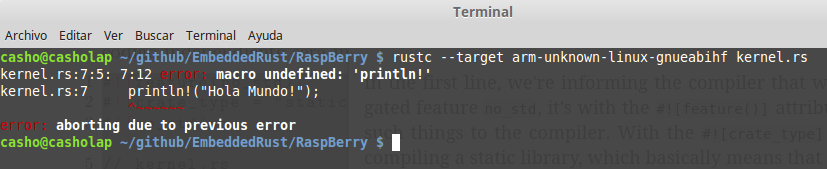
\includegraphics[width=1\linewidth]{rust_kernel1.png}
	\caption{Resultados de la compilación cruzada}
	\label{fig0001}
\end{figure}

Como se muestra en la figura \ref{fig0001}, la macro \textbf{println!} no está definida, porque no esta implementada en las rutinas de E/S y el runtime, ¡somos independientes!. Si removemos la instrucción \textbf{println!} e intentamos compilar nuevamente obtenemos lo mostrado en la figura \ref{fig0002}

\begin{figure}
	\centering	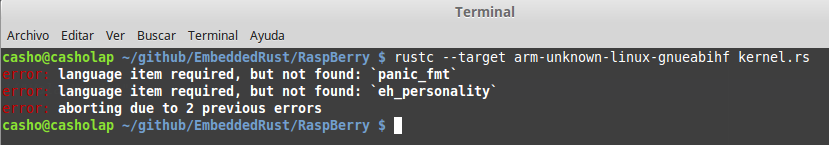
\includegraphics[width=1\linewidth]{rust_kernel2.png}
	\caption{compilación cruzada sin \textbf{println!}}
	\label{fig0002}
\end{figure}

Esto significa que el runtime mínimo de Rust espera que estas dos funciones sean definidas. Ambas funciones son usadas por los mecanismos de falla/manejo del compilador. Para un \textit{hola mundo} independiente, definimos estos como implementaciones independientes.

\begin{lstlisting}[language=erlang]
// kernel.rs
#![feature(no_std, lang_items)]
#![crate_type = "staticlib"]
#![no_std]

pub extern fn main() {  
    loop {}
}

#[lang = "eh_personality"]
extern fn eh_personality() {}

#[lang = "panic_fmt"]
extern fn panic_fmt() {}  
\end{lstlisting}

El atributo \textbf{\#[lang]} informa al compilador que la función esta siendo definida para el runtime. Ya que este atributo es una característica necesitamos agregarla a nuestra lista en el atributo \textbf{\#![feature()]}. Ahora para compilar, necesitamos informarle al compilador que queremos producir un archivo objeto. Un archivo objeto es básicamente el código compilado con los símbolos definidos. Usaremos el archivo objeto generado para enalzarlos con \textbf{arm-none-eabi-gcc} y generar el archivo \textbf{kernel.elf}. Adicionamos la bandera \textbf{-O} para remover algunos símbolos innecesarios y realizar alguna optimización. Tambien cambiamos nuestra función \textbf{main} para que sea pública y externa.  Esto informa al compilador que nuestra función será usado externamente.
\begin{lstlisting}[language=bash]
rustc --target arm-unknown-linux-gnueabihf -O --emit=obj kernel.rs
\end{lstlisting}

Esto genera el archivo \textbf{kernel.o}. Podemos comprobar si nuestro compilador cruzado esta trabajando y produciendo código máquina compatible con ARM utilizando el comando \emph{file}:

\begin{lstlisting}[language=bash]
file kernel.o
#kernel.o: ELF 32-bit LSB  relocatable, ARM, EABI5 version 1 (SYSV), not stripped
\end{lstlisting}

Podemos revisar los símbolos del archivo objeto usando \textbf{arm-none-eabi-nm}\footnote{si el comando anterior no funciona, es necesario intalar lo siguiente: sudo apt-get install binutils-arm-none-eabi} :

\begin{lstlisting}[language=bash]
arm-none-eabi-nm kernel.o
\end{lstlisting}

Lo cual produce el resultado de la figura \ref{fig0003}.

\begin{figure}
	\centering	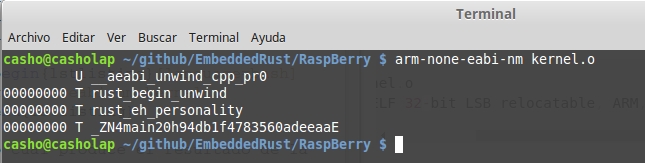
\includegraphics[width=1\linewidth]{rust_kernel3.png}
	\caption{Etiquetas del \textbf{kernel.o}}
	\label{fig0003}
\end{figure}

Esto nos muestra los tres símbolos definidos por nuestro código fuente . El extraño es nuestra función principal \textbf{main}. Esto sucede debido a algo que se llama renombrado, que es algo que el compilador hace para evitar conflictos de nombres. Queremos que nuestros símbolos sean claros, por lo que las herramientas externas sabe cómo hacer referencia a ella. Para indicar al compilador que no destrozar nuestra función principal , tenemos que indicarlo :

\begin{lstlisting}[language=erlang]
// kernel.rs
#![feature(no_std, lang_items)]
#![crate_type = "staticlib"]
#![no_std]

#[no_mangle]
pub extern fn main() {  
    loop {}
}

#[lang = "eh_personality"]
extern fn eh_personality() {}

#[lang = "panic_fmt"]
extern fn panic_fmt() {}  
\end{lstlisting}

Si compilamos y checamos los símbolos obtenemos lo indicado en la figura \ref{fig0004}

\begin{figure}
	\centering	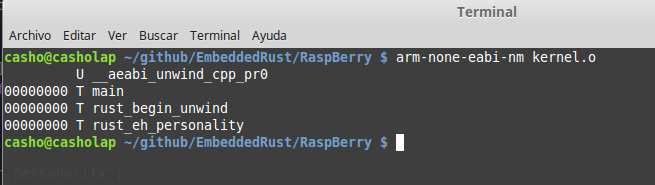
\includegraphics[width=1\linewidth]{rust_kernel4.png}
	\caption{Etiquetas del \textbf{kernel.o} con \textbf{no\_mangle}}
	\label{fig0004}
\end{figure}

Ahora todos las etiquetas son claras lo cual será útil cuando lo necesitemos llamar desde el ensamblador.

\subsection{Haciendo el LED parpadear}

La dirección base de la Raspberry Pi B+ GPIO es 0x20200000. El registro que nos permitirá encender nuestro LED es la dirección base + offset 0x8 y tenemos que establecer el bit 15 al 1 para encenderlo. Para desactivarlo, tenemos que establecer el bit 15 al 1 en la dirección base + 0xB offset. Entre estos cambios , tenemos que bloquear el programa durante algún tiempo. Nuestro código se verá así :

\begin{lstlisting}[language=erlang]
// kernel.rs

#![feature(no_std, lang_items, asm)]
#![crate_type = "staticlib"]
#![no_std]

const GPIO_BASE: u32 = 0x20200000;

fn sleep(value: u32) {  
    for _ in 1..value {
        unsafe { asm!(""); }
    }
}

#[no_mangle]
pub extern fn main() {  
    let gpio = GPIO_BASE as *const u32;
    let led_on = unsafe { gpio.offset(8) as *mut u32 };
    let led_off = unsafe { gpio.offset(11) as *mut u32 };

    loop {
        unsafe { *(led_on) = 1 << 15; }
        sleep(500000);
        unsafe { *(led_off) = 1 << 15; }
        sleep(500000);
    }
}

#[lang = "eh_personality"] extern fn eh_personality() {}
#[lang = "panic_fmt"] extern fn panic_fmt() {}
\end{lstlisting}

Hemos añadido una función de apagado automático que básicamente es un bucle vacío para un rango dado. El \textbf{unsafe { asm!(" ")}} fue la manera que se ha encontrado para evitar que el compilador para elimine a esta parte del código durante la fase de optimización, ya que no parece hacer nada. En la función principal \textbf{main}, creamos un puntero raw para la dirección de GPIO\_BASE, entonces obtenemos un puntero mutable de los lugares que queremos cambiar, que son el uno para encender el LED y para apagarlo. Desde la llamada desplazamiento implica la eliminación de referencias un puntero raw, esto es una operación insegura, por tanto, los bloques no seguros. Con que sólo podemos hacer un bucle infinito que Enciende el LED, espera, apagarlo y esperar.

\subsection{Preparando el codigo }

Ahora podemos compilar el codigo para ejecutarlo en la Raspberry:

\begin{lstlisting}[language=bash]
rustc --target arm-unknown-linux-gnueabihf -O --emit=obj kernel.rs
\end{lstlisting}

Con el archivo \textbf{kernel.o} generado se necesita enlazar el código usando \textbf{arm-none-eabi-gcc},  asi que esto puede configurar nuestro símbolo \textbf{main} como el punto de  entrada a nuestro programa, para generar el archivo kernel.elf y luego usar \textbf{arm-none-eabi-objcopy} para generar el archivo binario final \textbf{kernel.img} \footnote{Si la instrucción de la linea 1 no se ejecuta es necesario intalar con el siguiente comando: sudo apt-get install gcc-arm-none-eabi} .
\begin{lstlisting}[language=bash]
arm-none-eabi-gcc -O0 -mfpu=vfp -mfloat-abi=hard -march=armv6zk -mtune=arm1176jzf-s -nostartfiles kernel.o -o kernel.elf
arm-none-eabi-objcopy kernel.elf -O binary kernel.img
\end{lstlisting}
Con nuestro kernel.img construido , sólo tenemos que copiarlo en nuestra frambuesa SD junto con los otros archivos de arranque ( start.elf y bootcode.bin ) , se adhieren a nuestra micro SD de nuevo en el Pi de frambuesa y encenderlo para ver nuestra pequeña núcleo en ejecución y parpadea el LED !

Hay un montón de otras cosas interesantes que podemos hacer , como usar el temporizador del sistema en chip para poner en práctica nuestra función dormir o crear algunas abstracciones de la parte superior de la GPIO se dirige para encapsular todas las llamadas inseguras en una API más elegante . Pero creo que por ahora esto es una buena manera de empezar con la programación de metal desnudo con moho .
\chapter{Sistema Operativo para x86}

En este caso se necesitan tres archivos:
\begin{itemize}
\item boot.s.- Punto de entrada del kernel que configura el entorno del procesador
\item kernel.rs.- Las rutinas actuales del kernel
\item linker.ld.- Para enlazar los archivos anteriores 
\end{itemize}


Les presento el nuevo sistema operativo UtVitam. UtVitam es un sistema operativo enfocado a dar vida a nuevos proyectos que busquen funcionar independiente y embebidos, por ello es que UtVitam proviene del latin que significa \textbf{A la vida}. La primera decisión que debemos hacer nada más plantearnos el sistema operativo es ¿cuál va a ser el bootloader?

Aquí existen múltiples variantes, e incluso podríamos crear uno nosotros; sin embargo, vamos a usar GRUB, porque la mayoría conoce más o menos algo de él. Creamos una carpeta que será el root de nuestro sistema operativo y allí creamos la carpeta /boot/grub

\begin{lstlisting}[language=bash]
mkdir UtVitamroot && cd UtVitamroot
mkdir -p boot/grub
\end{lstlisting}

Allí creamos el fichero grub.cfg de la siguiente manera:

\begin{lstlisting}[language=bash]
menuentry "UtVitam" {

echo "Booting UtVitam"

multiboot /Ut/START.ELF

boot

}
\end{lstlisting}


En este fichero hemos visto como GRUB cargará nuestro kernel, en este caso, en /Ut/START.ELF. Ahora debemos crear nuestro kernel.

Para ello necesitaremos el GCC y GAS (el ensamblador del proyecto GNU, suele venir con el gcc). Así pues vamos a crear el kernel.

Primero hacemos un archivo llamado kernel.asm. Este archivo contendrá el punto de inicio de nuestro kernel y además definirá el multiboot (una característica de algunos bootloaders como GRUB). El contenido de kernel.asm será:

\begin{lstlisting}[language=bash]
.text

.globl start

start:

jmp multiboot_entry

.align 4

multiboot_header:

.long 0x1BADB002

.long 0x00000003

.long -(0x1BADB002+0x00000003)

multiboot_entry:

movl $(stack + 0x4000), %esp

call UtVitam_Main

loop: hlt

jmp loop

.section ".bss"

.comm stack,0x4000

\end{lstlisting}

Todo lo relacionando con multiboot es simplemente seguir la especificación nada más. Todo empezará en start, llamará a multiboot\_entry, habremos definido el multiboot header en los primeros 4k y lo pondremos (con movl).


Más tarde llamamos a UtVitam\_Main que es nuestra función en C del kernel. En el loop hacemos un halt para parar el ordenador. Esto se compila con:

\begin{lstlisting}[language=bash]
as -o kernel.o -c kernel.asm
\end{lstlisting}

Ahora vamos a entrar a programar en C. Pensarás que ahora todo es pan comido, ponemos un printf en main y ya está, lo hemos hecho.

Pues no, ya que printf y main son funciones que define el sistema operativo, ¡pero nosotros lo estamos creando! Solo podremos usar las funciones que nosotros mismos definamos.

En capítulos posteriores hablaré de como poner nuestra propia libraría del C (glibc, bionic, newlibc) pero tiempo al tiempo. Hemos hablado que queremos poner texto en pantalla, bueno veremos como lo hacemos.

Hay dos opciones, una es llamar a la BIOS y otra es manejar la memoria de la pantalla directamente. Vamos a hacer esto último pues es más claro desde C y además nos permitirá hacerlo cuando entremos en modo protegido.

Creamos un fichero llamado UtVitam\_Main.c con el siguiente contenido:

\begin{lstlisting}[language=C++]
int UtVitam_Main()

{

char *str = "NextDivel says Hello World", *ch;

unsigned short *vidmem = (unsigned short*) 0xb8000;

unsigned i;

for (ch = str, i = 0; *ch; ch++, i++)

vidmem[i] = (unsigned char) *ch | 0x0700;

return 0;

}
\end{lstlisting}

Con esto manipulamos directamente la memoria VGA y caracter a caracter lo vamos escribiendo. Compilamos desactivando la stdlib:

\begin{lstlisting}[language=bash]
gcc -o UtVitam_Main.o -c UtVitam_Main.c -nostdlib -fPIC -ffreestanding
\end{lstlisting}


Si has llegado hasta aquí querrás probar ya tu nuevo y flamante sistema operativo, pero todavía no hemos terminado. Necesitamos un pequeño fichero que diga al compilador en que posición del archivo dejar cada sección. Esto se hace con un linker script. Creamos link.ld:

\begin{lstlisting}[language=C++]
ENTRY(start)

SECTIONS

{

. = 0x00100000;

.multiboot_header :

{

*(.multiboot_header)

}

.text :

{

code = .; _code = .; __code = .;

*(.text)

. = ALIGN(4096);

}

.data :

{

data = .; _data = .; __data = .;

*(.data)

*(.rodata)

. = ALIGN(4096);

}

.bss :

{

bss = .; _bss = .; __bss = .;

*(.bss)

. = ALIGN(4096);

}

end = .; _end = .; __end = .;

}
\end{lstlisting}

Con esto definimos la posición de cada sección y el punto de entrada, start, que hemos definido en kernel.asm. Ahora ya podemos unir todo este mejunje:

\begin{lstlisting}[language=bash]
gcc -o START.ELF kernel.o UtVitam_Main.o -Tlink.ld -nostdlib -fPIC -ffreestanding -lgcc
\end{lstlisting}

Ahora copiamos START.ELF al /next dentro de nuestra carpeta que simula el root de nuestro sistema operativo. Nos dirigimos a la carpeta root de nuestro sistema operativo nuevo con la consola y verificamos que hay dos archivos: uno /boot/grub/grub.cfg y otro /Ut/START.ELF.

Vamos al directorio superior y llamamos a una utilidad de creación ISOs con GRUB llamada grub-mkrescue

\begin{lstlisting}[language=bash]
grub-mkrescue -o UtVitam.iso UtVitamroot
grub-mkrescue -d /usr/lib/grub/i386-pc/ -o os.iso isofiles
\end{lstlisting}


Una vez hayamos hecho esto tendremos una ISO. Esta ISO puede abrirse en ordenadores x86 (64 bits también) y máquinas virtuales. Para probarlo, voy a usar QEMU. Llamamos a QEMU desde la línea de comandos:

\begin{lstlisting}[language=bash]
qemu-system-i386 nextdivel.iso

\end{lstlisting}

Arrancará SeaBIOS y más tarde tendremos GRUB. Después si todo va correcto veremos nuestra frase.


\bibliographystyle{acm}
\bibliography{../bibliografia}
\end{document}
